\chapter{Lattice Correlators}

In Section 4 we discussed the reduction of the pion 2-point correlation
function to a product of quark propagators and possibly gauge links, and its
relation to sum over states from which $M_\pi$ and $f_\pi$ can be extracted.
Here I enlarge the discussion to general 2-point and 3-point functions.
Consider the calculation of the matrix element $\langle K^+|V_\mu|D^0\rangle$
which arises in the extraction of semi-leptonic form factors.  The 3-point
correlation function needed to calculate this ME is
\begin{equation}
\begin{aligned}
C_\mu^{PVP}(t_x, p; t_y, q) &=
\sum_{x,y} e^{-i(q\cdot y+p\cdot x)}\, T[K^+ V_\mu D^0] \\
&= \sum_{x,y} e^{-i(q\cdot y+p\cdot x)}\,
   \bar{s}(0)\gamma_5 u(0)\;\bar{c}(y)\gamma_\mu s(y)\;\bar{u}(x)\gamma_5 c(x) \\
&= \sum_{x,y} e^{-i(q\cdot y+p\cdot x)}\,
   \gamma_5 S_F^u(x,0)\gamma_5 S_F^s(0,y)\gamma_\mu S_F^u(y,x) \\
&\sim \frac{\exp(-E_K(p+q)t_y - E_D(p)(t_x-t_y))}{4E_K(p+q)E_D(p)}
   \langle 0|\bar{u}\gamma_5 s|K(p+q)\rangle \\
&\qquad \times \langle K(p+q)|\bar{s}\gamma_\mu c|D(p)\rangle
   \langle D(p)|\bar{c}\gamma_5 u|0\rangle .
\end{aligned}
\end{equation}

\begin{figure}[htbp]
\centering
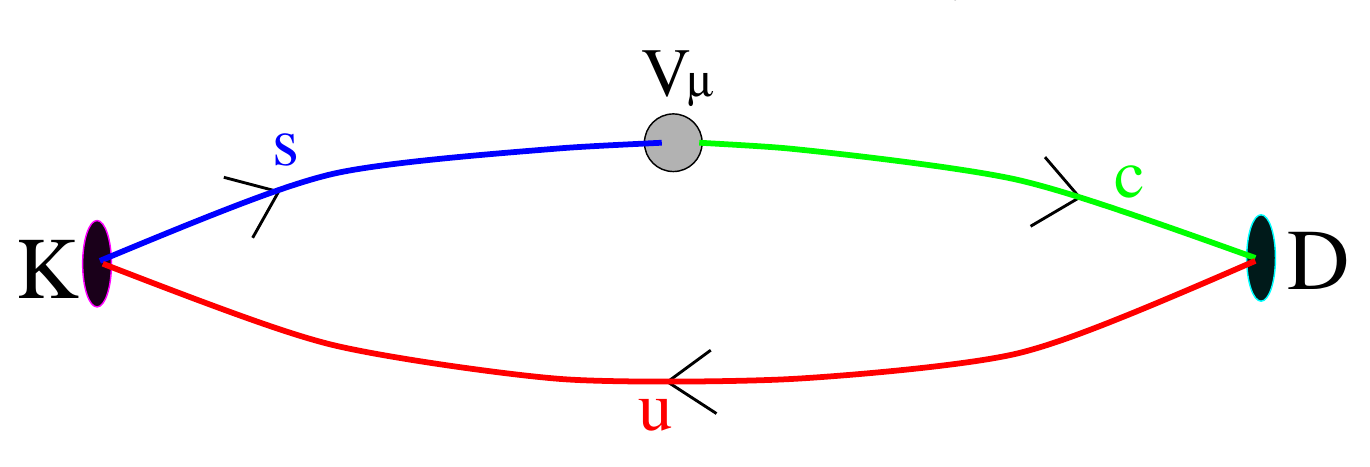
\includegraphics[width=0.8\textwidth]{images/fig20.png}
\caption{Schematic of Feynman diagram for $KV_\mu D$ in terms of $c$, $s$, and
$u$ quark propagators.}
\label{fig:20}
\end{figure}

I have used (i) Wick contractions to express the correlation function in terms
of quark propagators $S_F$ (see Fig.~20); (ii) local bilinears for the source
and sink operators and the vector current (to improve the signal one usually
uses smeared operators and an improved current); and (3) the interpolating
operator for the $D$ meson and the current insertion are at definite momentum.
Momentum conservation then fixes $p_k$.  The final form in Eq.~17.2 shows the
behavior for large Euclidean time separations ($t_x \ll t_y \ll t_0$).  Of the
many terms in the right hand side, we are only interested in the matrix element
$\langle K(p+q)|\bar{c}\gamma_\mu s|D(p)\rangle$.  The remaining factors can
all be extracted from 2-point correlation functions.  Thus, one can make
individual fits to all the required correlators, or design a ratio in which the
maximum number of unwanted factors cancel.  In practice, to improve the
numerical signal, a single fit is made to a ratio of 3-point to a combination
of 2-point functions, $T[KV_\mu D]/(T[KK]\,T[DD])$, that gets rid of the
exponential in time behavior.

To make fits to such correlation functions projected on to definite spatial
momenta, we have to address three questions:
\begin{itemize}
\item Is the correlator even or odd in its time variables?
\item Is the correlator even or odd in its momenta?
\item Is the correlator real or imaginary?  As mentioned before only the real
part of Euclidean correlation functions has a signal.
\end{itemize}

In practice we usually work in terms of bilinear operators given in Table~8
where factors of $i$ have been dropped for brevity.  In this basis of operators
one needs to know whether a given $n$-point function has a signal in the real
or imaginary part.  To answer these questions we use the discrete symmetries,
$T$, $P$, and $CPH$ discussed in Table~2 and in Eq.~10.11.  For each element of
the Dirac algebra, $\Gamma_A$ define three signs, $\tau_A$, $\pi_A$, and
$\chi_A$, associated with $T$, $P$, and $CPH$:
\begin{equation}
\begin{aligned}
\gamma_4\gamma_5\Gamma_A\gamma_5\gamma_4 &= \tau_A\Gamma_A;\\
\gamma_4\Gamma_A\gamma_4 &= \pi_A\Gamma_A;\\
C\gamma_4\gamma_5\Gamma_A\gamma_5\gamma_4 C^{-1} &= \chi_A\Gamma_A^* .
\end{aligned}
\end{equation}

\begin{table}[htbp]
\centering
\begin{tabular}{lcccccccc}
\toprule
 & $1$ & $\gamma_i$ & $\gamma_4$ & $\gamma_i\gamma_j$ & $\gamma_i\gamma_4$ & $\gamma_i\gamma_5$ & $\gamma_4\gamma_5$ & $\gamma_5$ \\
\midrule
$\tau_A$ & $+$ & $+$ & $-$ & $+$ & $-$ & $-$ & $+$ & $-$ \\
$\pi_A$ & $+$ & $-$ & $+$ & $+$ & $-$ & $+$ & $-$ & $-$ \\
$\chi_A$ & $+$ & $-$ & $+$ & $+$ & $-$ & $+$ & $-$ & $-$ \\
\bottomrule
\end{tabular}
\caption{The signs for bilinear currents under $T$, $P$ and $CPH$
transformations.}
\label{tab:7}
\end{table}

These signs are given in Table~7 and the application to 2-point and 3-point
correlators is illustrated in the next two sub-sections.

\section{Two-point meson correlators}

Consider the general two-point correlator
\begin{equation}
\begin{aligned}
C^{BA}(p,t) &= \sum_x e^{-ip\cdot x}\,
   \langle \bar{\psi}_2(x)\Gamma_B\psi_1(x)\;\bar{\psi}_1(0)\Gamma_A\psi_2(0)\rangle ,\\
&= -\sum_x e^{-ip\cdot x}\,
   \mathrm{Tr}\big(S_2(0,x)\Gamma_B S_1(x,0)\Gamma_A\big) ,
\end{aligned}
\end{equation}

where Tr is trace over spin and color indices and $t \equiv x_4$.  $T$, $P$ and
$CPH$ then imply the following:
\begin{itemize}
\item If $\tau_A\tau_B = \pm 1$, $C^{BA}(p,t)$ is even (odd) in $t$.
\item If $\pi_A\pi_B = \pm 1$, $C^{BA}(p,t)$ is even (odd) in $p$.
\item If $\chi_A\chi_B = \pm 1$, $C^{BA}(p,t)$ is real (imaginary).
\end{itemize}

Note that in Eq.~17.3 the second quark propagator is from $x \to 0$.  Using the
hermiticity property $S(x,0) = \gamma_5 S(0,x)^\dagger \gamma_5$ we can write
this in terms of $S(x,0)$.  This simple property, the relation between the
quark propagator from a given point and the anti-quark propagator to that
point, leads to a huge computational saving.  For example, if the momentum
projection is done by summing over the $L^3$ sink points $x$ with weight
$\exp(ip\cdot x)$, then, because of the hermiticity property we need only one
propagator inversion instead of $L^3+1$.

\section{Interpolating operators}

For Wilson-like fermions the interpolating field operators for mesons and
baryons at zero-momentum are given in Table~8.  The three flavors are labeled
$u$, $d$, $s$ for brevity.  The baryon operators need further clarification as
discussed in [156] and reproduced below.

\begin{table}[htbp]
\centering
\begin{tabular}{lll}
\toprule
State & $I^G(J^{PC})$ & Operator \\
\midrule
Scalar ($\sigma$) & $1^-(0^{++})$ & $u(x)d(x)$ \\
                  & $1^-(0^{++})$ & $u(x)\gamma_4 d(x)$ \\
Pseudoscalar      & $1^-(0^{-+})$ & $u(x)\gamma_5 d(x)$ \\
                  & $1^-(0^{-+})$ & $u(x)\gamma_4\gamma_5 d(x)$ \\
Vector            & $1^+(1^{--})$ & $u(x)\gamma_i d(x)$ \\
                  & $1^+(1^{--})$ & $u(x)\gamma_i\gamma_4 d(x)$ \\
Axial ($a_1$)     & $1^-(1^{++})$ & $u(x)\gamma_i\gamma_5 d(x)$ \\
Tensor ($b_1$)    & $1^+(1^{+-})$ & $u(x)\gamma_i\gamma_j d(x)$ \\
\midrule
Nucleon octet     & $(\tfrac{1}{2},\tfrac{1}{2}^-)$ & $(u_a^T C d_b)\,\gamma_5 s_c\,\epsilon_{abc}$ \\
                  & $(\tfrac{1}{2},\tfrac{1}{2}^-)$ & $(u_a^T C\gamma_5 d_b)\,s_c\,\epsilon_{abc}$ \\
Delta decuplet    & $(\tfrac{3}{2},\tfrac{3}{2}^+)$ & $(u_a^T C\gamma_i d_b)\,s_c\,\epsilon_{abc}$ \\
\bottomrule
\end{tabular}
\caption{The local interpolating field operators for mesons and baryons in
Wilson-like theories.  Projection to zero momentum states is obtained by
summing over the points $x$ on a time slice.  The $C$-parity is only relevant
for flavor degenerate meson states.  The $(\ )$ in baryon operators denote
spin trace.  $C = \gamma_2\gamma_4$ and the symmetry properties of flavor
indices for nucleons are discussed in the text.  The decuplet baryon operator
is completely symmetric in flavor index.}
\label{tab:8}
\end{table}

The spin-1/2 baryons are created by the interpolating operators
\begin{equation}
O_{(ij)k} = (\psi_{a,i}^T C\gamma_5 \psi_{b,j})\,\psi_{c,k}\,\epsilon_{abc} ,
\end{equation}

where $a$, $b$ and $c$ label color, while $i$, $j$ and $k$ label flavor.  It
is simple to show that $O_{(ij)k} = -O_{(ji)k}$, so that there are only nine
independent operators---eight $SU(3)$ octets and the singlet
$\sum_{ijk}\epsilon_{ijk}O_{ijk}$.  One way to project against the singlet is
to form
\begin{equation}
B_{ijk} = O_{(ij)k} + O_{(ik)j} = B_{ikj} .
\end{equation}

There are eight independent $B_{ijk}$'s, the relation to the usual states being
exemplified by
\begin{equation}
\begin{aligned}
\sqrt{2}\,p &= -B_{duu} = 2B_{uud} = 2B_{udu},\\
\sqrt{2}\,\Sigma^+ &= -B_{suu} = 2B_{uus} = 2B_{usu},\\
\Sigma^0 &= B_{uds} + B_{dsu} = -B_{sud},\\
\sqrt{3}\,\Lambda^0 &= B_{uds} - B_{dsu}.
\end{aligned}
\end{equation}

The overall factor in these equations is arbitrary, while the relative
normalization is fixed by $SU(3)$ symmetry.  All spin-1/2 baryon correlators
are built out of the two contractions shown in Fig.~21.  The notation
$\langle DU\rangle_S = \langle UD\rangle_S$ corresponds to quarks of flavors
$U$ and $D$ contracted into a closed loop, while the propagator for $S$ carries
the spin quantum numbers of the baryon.  The notation $(DUS)$ corresponds to a
single ordered contraction of the three quarks.  We consider two types of
correlator, ``$\Sigma$-like'' and ``$\Lambda$-like''.  The former is
exemplified by that of the $\Sigma^0$

\begin{figure}[htbp]
\centering
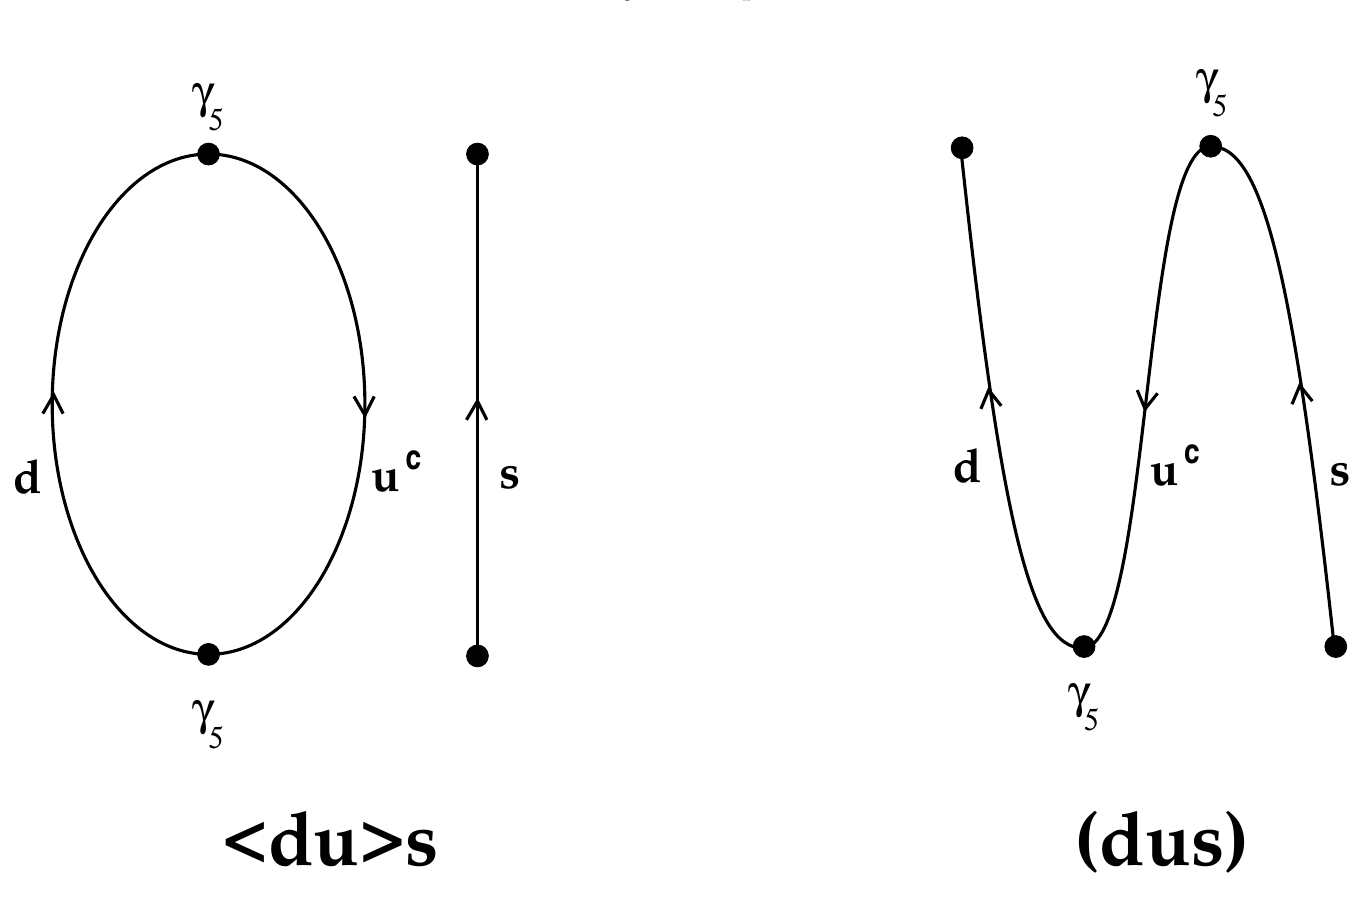
\includegraphics[width=0.8\textwidth]{images/fig21.png}
\caption{The two different types of contractions for the baryon states.}
\label{fig:21}
\end{figure}

\begin{equation}
S_{\{UD\}} = S_{\{DU\}} \equiv \langle B_{sud}(x)B_{sud}(0)\rangle
= \langle US\rangle_D + \langle DS\rangle_U + (USD) + (DSU) .
\end{equation}

This equation defines the sign conventions for the contractions.  The proton,
neutron, $\Sigma^+$, $\Sigma^-$, $\Xi^0$ and $\Xi^-$ correlators are also of
this type: they are, respectively, $D\{UU\}$, $U\{DD\}$, $S\{UU\}$, $S\{DD\}$,
$U\{SS\}$ and $D\{SS\}$.  The second type of correlator is that of the
$\Lambda^0$
\begin{equation}
\begin{split}
S_{[UD]} = S_{[DU]} &\equiv \tfrac{1}{3}\Big[\langle US\rangle_D + \langle DS\rangle_U + 4\langle UD\rangle_S\\
&\qquad - (USD) - (DSU) + 2(SUD) + 2(SDU) + 2(UDS) + 2(DUS)\Big] .
\end{split}
\end{equation}

When $m_u \neq m_d$, there is also a non-vanishing $\Lambda^0 - \Sigma^0$ cross
correlator, for which no useful results have been found [156].
Correlators of the form $A[AB]$ and $A\{AB\}$ are not independent---they are
related by
\begin{equation}
\begin{aligned}
A_{[AB]} &= \tfrac{1}{4}(3B_{[AA]} + B_{\{AA\}}),\\
A_{\{AB\}} &= \tfrac{1}{4}(B_{[AA]} + 3B_{\{AA\}}) .
\end{aligned}
\end{equation}

One can think of the results for the $A\{BB\}$ and $A[BB]$ masses as being
those for the $\Sigma$ and $\Lambda$, respectively, with $m_s = m_A$ and
$m_u = m_d = m_B$.  Unlike in the real world, there is nothing to stop
$m_A = m_B$.  Note, however, that in this case the $\Sigma$ and $\Lambda$ are
also degenerate, i.e.\ $M(A\{AA\}) = M(A[AA])$.  Indeed, the contractions in
the two cases are identical.

The interpretation of the results for the completely non-degenerate
correlators, $A[BC]$ and $A\{BC\}$, is more complicated.  Because isospin is
broken, the $\Sigma^0$- and $\Lambda$-like states mix, with both correlators
containing contributions from both physical states.  Let $M_+$ and $M_-$ be the
masses of the heavier and lighter states, respectively, and $\delta M$ the mass
difference.  At long times, the effective mass for both correlators will
asymptote to $M_-$.  However, at times short compared to the inverse mass
difference, i.e.\ $\delta M\,t_{\max} \ll 1$, there will be an approximate
plateau at a value which is a weighted average of the two masses.  The
surprising result, derived at lowest order in the chiral expansion in [156],
is that the masses extracted from these short time plateau are insensitive to
the isospin breaking and can be interpreted as those for $A[DD]$ and $A\{DD\}$
where $D = (B+C)/2$ is the mean mass for the two quarks.

\section{Three-point correlators}

A general three-point correlation function of meson operators and bilinear
currents has the form
\begin{equation}
\begin{aligned}
C^{CBA}(q,t_y;p,t_x) &= \sum_{x,y} e^{-i(q\cdot y+p\cdot x)}\,
   \langle \bar{\psi}_3(y)\Gamma_C\psi_2(y)\;\bar{\psi}_2(x)\Gamma_B\psi_1(x)
   \;\bar{\psi}_1(0)\Gamma_A\psi_3(0)\rangle ,\\
&= -\sum_{x,y} e^{-i(q\cdot y+p\cdot x)}\,
   \mathrm{Tr}\big(S_3(0,y)\Gamma_C S_2(y,x)\Gamma_B S_1(x,0)\Gamma_A\big) ,
\end{aligned}
\end{equation}

where $t_x \equiv x_4$ and $t_y \equiv y_4$.  $T$, $P$ and $CPH$ imply
\begin{itemize}
\item If $\tau_A\tau_B\tau_C = \pm 1$, $C^{CBA}(q,t_y;p,t_x)$ is even (odd)
under the simultaneous inversion of $t_x$ and $t_y$.
\item If $\pi_A\pi_B\pi_C = \pm 1$, $C^{CBA}(q,t_y;p,t_x)$ is even (odd) under
the simultaneous inversion of $p$ and $q$.
\item If $\chi_A\chi_B\chi_C = \pm 1$, $C^{CBA}(q,t_y;p,t_x)$ is real
(imaginary).
\end{itemize}

\section{CPS Symmetry}

The theory has an additional discrete symmetry, $CPS$, where $S$ is the
symmetry between switching $s$ and $d$ quarks [157].  This symmetry holds both
on the lattice and in the continuum for $m_d = m_s$.  For $m_d \neq m_s$ the
symmetry is softly broken, i.e., violations are proportional to $m_s - m_d$.
This symmetry plays a very useful role in the calculation of weak matrix
elements for it (i) restricts the set of possible Wick contractions, and (ii)
restricts the set of operators that mix with each other.

For a simple illustration consider $(\bar{s}\gamma_\mu Lu)(\bar{u}\gamma_\mu
Ld)$, a local 4-quark operator which is even under $CPS$
\begin{equation}
\begin{aligned}
(\bar{s}\gamma_\mu Lu)(\bar{u}\gamma_\mu Ld)
&\xrightarrow{P} (\bar{s}\gamma_4\gamma_\mu L\gamma_4 u)(\bar{u}\gamma_4\gamma_\mu L\gamma_4 d)\\
&\xrightarrow{C} (s^T C^{-1}\gamma_4\gamma_\mu L\gamma_4 C\bar{u}^T)(u^T C^{-1}\gamma_4\gamma_\mu L\gamma_4 C\bar{d}^T)\\
&= (s^T\gamma_4\gamma_\mu^T L\gamma_4\bar{u}^T)(u^T\gamma_4\gamma_\mu^T L\gamma_4\bar{d}^T)\\
&= (s^T\gamma_\mu^T R\bar{u}^T)(u^T\gamma_\mu^T R\bar{d}^T)\\
&= (\bar{u}R\gamma_\mu s)(\bar{d}R\gamma_\mu u)\\
&= (\bar{u}\gamma_\mu Ls)(\bar{d}\gamma_\mu Lu)\\
&\xrightarrow{S} (\bar{u}\gamma_\mu Ld)(\bar{s}\gamma_\mu Lu)
\end{aligned}
\end{equation}

The brackets denote trace over spin and color and the final reordering of the
two traced terms is allowed as time-ordering is implicit when calculating
expectation values.

This symmetry has a further generalization as discussed by Bernard and Soni in
[2,6].  For 4-fermion operators of the form $(\bar{\psi}_1\Gamma_A\psi_2)
(\bar{\psi}_3\Gamma_B\psi_4)$, there are two general switchings: (i)
$CPS'$ corresponding to $1 \leftrightarrow 2$ and $3 \leftrightarrow 4$, and
(ii) $CPS''$ corresponding to $1 \leftrightarrow 4$ and $2 \leftrightarrow 3$.
Bernard and Soni show in [2,6] how these switching symmetries are used to
restrict (i) the possible contractions in the decay $K \to \pi\pi$ via the
operator $(\bar{s}\gamma_\mu Lu)(\bar{u}\gamma_\mu Ld)$, and (ii) the mixing of
$O_\pm \equiv (\bar{s}\gamma_\mu Ld)(\bar{u}\gamma_\mu Lu) \pm
(\bar{s}\gamma_\mu Lu)(\bar{u}\gamma_\mu Ld) - (u \to c)$ with other operators.
I leave the details of these calculations as an exercise for the reader.
